%- block legend

\begin{wrapfigure}{l}{0.28\textwidth}
    \centering
    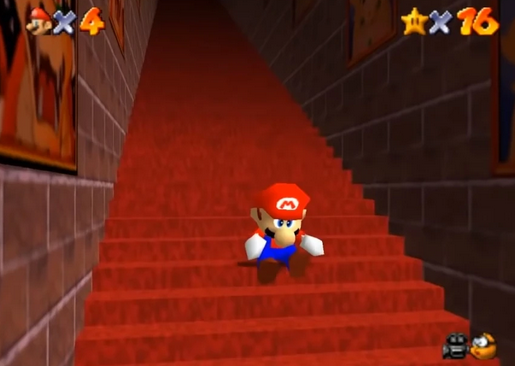
\includegraphics[width=0.28\textwidth]{mario.png}
\end{wrapfigure}

Você está jogando o clássico \textit{Super Mario 64}, e chegou em uma parte
estranha: há um corredor com uma escada que parece ser infinita...

Mas você descobriu um jeito de passar pela escada, explorando \sout{um bug} uma
técnica avançada de pulo. Se você conseguir acertar um pulo bem específico $K$
vezes seguidas, o final da escada finalmente aparece! Acertar o pulo,
entretanto, não é nada fácil.

Considere uma sequência de $N$ tentativas do pulo, feitas no instante 1, 2,
etc., até o instante $N$. A sequência é representada por uma string
$S$, de tamanho $N$, onde $S_i = $ \texttt{o} se a tentativa no instante $i$ foi acertada, e
$S_i = $ \texttt{x} se a tentativa no instante $i$ foi errada.

O final da escada aparece no primeiro instante em que se completa $K$ acertos seguidos.

Você deve processar $Q$ operações; em cada operação, troque (de
acerto para erro e vice-versa) a tentativa em um instante $i$ dado.
As mudanças feitas em uma operação se mantém para as operações seguintes.

Após cada operação, determine em que instante o final da escada aparece.

%- endblock

%- block input
A primeira linha contém três inteiros $N$, $K$ e $Q$
($1 \leq K \leq N \leq 10^5$, $1 \leq Q \leq 10^5$). A próxima linha contém a
string $S$ inicial. As próximas $Q$ linhas descrevem as operações a serem
feitas. Cada operação é descrita por um inteiro $i$ ($1 \leq i \leq N$)
indicando o instante a se mudar a tentativa.
%- endblock

%- block output
Após cada operação, imprima uma linha indicando em qual instante o final da
escada aparece. Se o final da escada não aparecer em nenhum instante, imprima
-1.
%- endblock

%- block notes
Considere o exemplo dado. Após a primeira operação, a string se torna \texttt{ooxooooxx}, e o final
aparece no instante 6. Após a segunda operação, a string se torna
\texttt{ooxxoooxx}, e o final aparece no instante 7. Após a terceira operação, a
string se torna \texttt{ooxxooxxx}, e o final da escada não aparece.
%- endblock

%- block editorial
This is the editorial.
%- endblock
